\documentclass[a4paper, 12pt]{article}\usepackage[utf8]{inputenc}
\usepackage[utf8]{inputenc}
\usepackage{xcolor, color, soul}
\usepackage{todonotes}
\usepackage{amsmath}
\usepackage{siunitx}
\usepackage{todonotes}
\usepackage{gensymb}
\usepackage{mathrsfs}
\usepackage{subcaption}
\usepackage{parskip}
\usepackage{xparse,mathtools}
\usepackage[hyphens]{url}
\usepackage{natbib}
\usepackage{float}
\usepackage{bbm}


\makeatletter
\newcommand*{\rom}[1]{\expandafter\@slowromancap\romannumeral #1@}
\makeatother
\usepackage{hyperref}
\hypersetup{
    colorlinks,
    citecolor=black,
    filecolor=black,
    linkcolor=black,
    urlcolor=black
}

\usepackage{listings}
\usepackage{color}
 



\definecolor{codegreen}{rgb}{0,0.6,0}
\definecolor{codegray}{rgb}{0.5,0.5,0.5}
\definecolor{codepurple}{rgb}{0.58,0,0.82}
\definecolor{backcolour}{RGB}{245,245,245}
 
\lstdefinestyle{mystyle}{
    backgroundcolor=\color{white},   
    commentstyle=\color{codegreen},
    keywordstyle=\color{blue},
    numberstyle=\tiny\color{codegray},
    stringstyle=\color{codepurple},
    basicstyle=\scriptsize,
    breakatwhitespace=false,         
    breaklines=true,                 
    captionpos=b,                    
    keepspaces=true,                 
    numbers=left,                    
    numbersep=4pt,                  
    showspaces=false,                
    showstringspaces=false,
    showtabs=false,                  
    tabsize=2
}

\lstset{style=mystyle}


\DeclarePairedDelimiterX{\rvect}[1]{[}{]}{\,\makervect{#1}\,}

\ExplSyntaxOn
\NewDocumentCommand{\makervect}{m}
 {
  \seq_set_split:Nnn \l_tmpa_seq { , } { #1 }
  \begin{matrix}
  \seq_use:Nn \l_tmpa_seq { & }
  \end{matrix}
 }
\ExplSyntaxOff
 



\begin{document}
%----------------------------------------------------------------------------------------
%	TITLE PAGE
%----------------------------------------------------------------------------------------

\begin{titlepage} % Suppresses displaying the page number on the title page and the subsequent page counts as page 1
	\newcommand{\HRule}{\rule{\linewidth}{0.5mm}} % Defines a new command for horizontal lines, change thickness here
	
	\center % Centre everything on the page
	
	%------------------------------------------------
	%	Headings
	%------------------------------------------------
	
	\textsc{\LARGE TTK4135 Optimization and Control}\\[1.5cm] % Main heading such as the name of your university/college
	
	%\textsc{\Large Major Heading}\\[0.5cm] % Major heading such as course name
	
	\textsc{\large }\\[0.5cm] % Minor heading such as course title
	
	%------------------------------------------------
	%	Title
	%------------------------------------------------
	
	\HRule\\[0.4cm]
	
	{\huge\bfseries Helicopter Lab Report}\\[0.4cm] % Title of your document
	
	\HRule\\[1.5cm]
	
	%------------------------------------------------
	%	Author(s)
	%------------------------------------------------
	
	\begin{minipage}{0.4\textwidth}
		\large
		\textit{Student numbers}\\
		\textsc{768455}\\ % Supervisor's name
		\textsc{768632}\\
		\textsc{768706}
	\end{minipage}
	
	% If you don't want a supervisor, uncomment the two lines below and comment the code above
	%{\large\textit{Author}}\\
	%John \textsc{Smith} % Your name
	
	%------------------------------------------------
	%	Date
	%------------------------------------------------
	
	\vfill\vfill\vfill % Position the date 3/4 down the remaining page
	
	{\large\today} % Date, change the \today to a set date if you want to be precise
	
	%------------------------------------------------
	%	Logo
	%------------------------------------------------
	
	%\vfill\vfill
	%\includegraphics[width=0.2\textwidth]{placeholder.jpg}\\[1cm] % Include a department/university logo - this will require the graphicx package
	 
	%----------------------------------------------------------------------------------------
	
	\vfill % Push the date up 1/4 of the remaining page
	
\end{titlepage}












%\maketitle

%----------------------------------------------------------------------
%//////////////////////////////////////////////////////////////////////
%----------------------------------------------------------------------
\clearpage
\begin{abstract}

This report is for the helicopter lab in the course TTK4135 Optimization and Control. The purpose of the project is to derive a model for the helicopter system and control it using different types of optimal controllers. This report also covers how the different optimizations of the system were found.


\end{abstract}

\clearpage

%----------------------------------------------------------------------
%//////////////////////////////////////////////////////////////////////
%----------------------------------------------------------------------

\tableofcontents
\phantomsection
\clearpage

%----------------------------------------------------------------------
%//////////////////////////////////////////////////////////////////////
%---------------------------------------------------------------------

\section{Introduction}


This report covers a laboratory exercise about optimal control of a helicopter system. A model for the helicopter is given in the assignment, and the control program is made in MATLAB and Simulink. The overall goal of the laboratory exercise is to combine several different control layers to achieve a desired behaviour. The starting point is a basic control layer alone, consisting of a PD-controller for the pitch and a PID-controller for the elevation. This control system is then extended with an additional optimization layer, and furthermore an additional advanced control layer using LQR and feedback. The final control hierarchy takes advantage of the combination of different control approaches in order to cancel individual weaknesses of each approach.


The report is divided in three main parts corresponding to the parts of the assignment. Implementation of the different controllers is done using MATLAB and Simulink. The Simulink models, plots and MATLAB script are in separate appendixes.


%----------------------------------------------------------------------
%//////////////////////////////////////////////////////////////////////
%---------------------------------------------------------------------

\section{System Description}

The mathematical model used in this assignment is summarized by the following equations

\begin{subequations}\label{model_eq}
    \begin{equation}
        \ddot{e}+K_3K_{ed}\dot{e}+K_3K_{ep}e=K_3K_{ep}e_c
    \end{equation}
    \begin{equation}
        \ddot{p} +K_1K_{pd}\dot{p}+K_1K_{pp}p=K_1K_{pp}p_c
    \end{equation}
    \begin{equation}
        \dot{r}=-K_2p
    \end{equation}
\end{subequations}

Parameter values, variables and description is given in in the following tables
\begin{table}[h]
    \centering
    \caption{Variables}
    \label{tab:symbol}
    \begin{tabular}{ll}
        \hline
        \textit{Symbol}&\textit{Definition}\\
        \hline
        $p$ & Pitch\\
        $p_c$ & Setpoint for pitc\\
        $\lambda$ & Travel\\
        $r$ & Speed of travel\\
        $r_c$ & Setpoint for speed of travel\\
        $e$ & Elevation\\
        $e_c$ & Setpoint for elevation\\
        $V_f$ & Voltage, motor in front\\
        $V_b$ & Voltage, motor in back\\
        $V_d$ & Voltage difference, $V_f-V_b$\\
        $V_s$ & Voltage sum, $V_f+V_b$\\
        $K_{pp}, K_{pd}, K_{ep}, K_{ei}, K_{ed}$ & Controller gains\\
        $T_g$ & Moment needed to keep the helicopter flying\\ 
        \hline
    \end{tabular}
\end{table}

\begin{table}[h]
    \centering
    \caption{Paramteres and values}
    \label{tab:symbol}
    \begin{tabular}{llll}
        \hline
        \textit{Symbol}&\textit{Definition}&\textit{Value}&\textit{Unit}\\
        \hline
        $l_a$ & Distance from elevation axis to the helicopter body & 0.63 & m\\
        $l_h$ & Distance from pitch axis to motor & 0.18 & m\\
        $K_f$ & Force constant motor & 0.25 & N/V\\
        $J_e$ & Moment of inertia for elevation & $0.83$ & $kg m^2$\\
        $J_t$ & Moment of inertia for travel & $0.83$ & $kg m^2$\\
        $J_p$ & Moment of inertia for pitch & $0.034$ & $kg m^2$\\
        $m_h$ & Mass of helicopter & 1.05 & kg\\
        $m_w$ & Balance weight & 1.87 & kg\\
        $m_g$ & Effective mass of the helicopter & 0.05 & kg\\
        $K_p$ & Force to lift the helicopter from the ground & 0.49 & N\\
        \hline
    \end{tabular}
\end{table}

\clearpage

\section{Part 2: Optimal Control of Pitch/Travel without Feedback}

In this part the elevation is being disregarded to find an optimal trajectory $X^*$ and corresponding optimal input sequence without the use of feedback $u^*$ that moves the helicopter 180 degrees.

\subsection{The Continuous State Space Form}
A model on continuous state space form with several states and scalar input has the following format. 

\begin{equation}
    \boldsymbol{\dot{x}} = \boldsymbol{A_c}\boldsymbol{x} + \boldsymbol{B_c} u
\end{equation}

In the assignment the following state vector and control input (\ref{state_vec_and_input}) is given together with the model equations in \ref{eq:model_eqs}.

\begin{equation} \label{state_vec_and_input}
    \boldsymbol{x} = 
    \begin{bmatrix}
        \lambda\\
        r\\
        p\\
        \dot{p}\\
    \end{bmatrix},
    \begin{tabular}{cc}
         &  \\
         & 
    \end{tabular}
    u=p_c
\end{equation} 

\begin{subequations}\label{eq:model_eqs}
    \begin{equation}
        \dot{\lambda}=r
    \end{equation}
    \begin{equation}
        \ddot{p}=K_1K_{pp}(p_c-p)-K_{pd}\dot{p}
    \end{equation}
    \begin{equation}
        \dot{r}=-K_2p
    \end{equation}
\end{subequations}


These are used to derive the following state space matrices:

\begin{equation}
     \boldsymbol{A_c}=\begin{bmatrix}
    0 & 1 & 0 & 0\\
    0 & 0 & -K_2 & 0\\
    0 & 0 & 0 & 1\\
    0 & 0 & -K_1K_{pp} & -K_{1}K_{pd}\\
    \end{bmatrix}
    \begin{tabular}{cc}
         &  \\
         & 
    \end{tabular}
    \boldsymbol{B_c}=\begin{bmatrix}
    0\\
    0\\
    0\\
    K_1K_{pp}\\
    \end{bmatrix} 
\end{equation}

Hence, the model on continuous state space form can be written as shown below (\ref{eq:cont_state_space}). 

\begin{equation} \label{eq:cont_state_space}
    \begin{bmatrix}
        \dot{\lambda}\\
        \dot{r}\\
        \dot{p}\\
        \ddot{p}\\
    \end{bmatrix}
    = \begin{bmatrix}
    0 & 1 & 0 & 0\\
    0 & 0 & -K_2 & 0\\
    0 & 0 & 0 & 1\\
    0 & 0 & -K_1K_{pp} & -K_{1}K_{pd}\\
    \end{bmatrix}
    \begin{bmatrix}
        \lambda\\
        r\\
        p\\
        \dot{p}\\
    \end{bmatrix}
    + \begin{bmatrix}
    0\\
    0\\
    0\\
    K_1K_{pp}\\
    \end{bmatrix} p_c
\end{equation}

Figure \ref{fig:chart_2.1} is given in the lab assignment and illustrates the layers in the control hierarchy used in this section of the assignment. The derived model (\ref{eq:cont_state_space} does not only model the helicopter, referred to as the physical layer in the figure, but also the basic control layer. This includes the pitch controller (PD) and the elevation controller (PID). The integration of these controllers into the model is recognizable through the appearance of $K_{pp}$ and $K_{pd}$ in the model equations. The optimization layer on the other hand is not a part of the model. Instead, this layer \textit{uses} the model in its calculations. The optimization layer is covered more in depth in section \ref{3.3}.

------------------------------------------------

As figure \ref{fig:chart_2.1} shows, there is no feedback from the model back to the optimization layer. Hence, this layer is based on the model only. In practice, the model is used to calculate an optimal trajectory for moving the helicopter a desired path. In addition, a corresponding optimal input sequence is calculated using the same model. The goal of this input sequence is to provoke the desired behaviour given by the optimal trajectory.

The state vector in this model consist of travel, travel rate, pitch and pitch rate. The model is thus derived assuming no interaction between the elevation and the modeled states. However interactions between these variables are present and may lead to small deviations between estimations based on the model and the real system. This will not be a significant problem as long as the elevation is at a height around zero. If it is much higher or lower the travel radius will decrease, but the control sequence will stay the same. This can for instance result in the helicopter traveling too far


\begin{figure}[H]
    \centering
    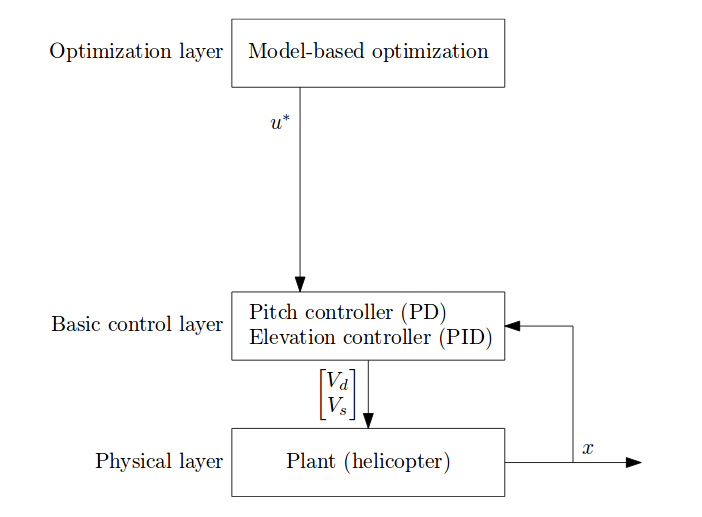
\includegraphics[width=140mm]{Part2/fig7_oppg.png}
    \caption{Control hierarchy}
    \label{fig:chart_2.1}
\end{figure}

 \subsection{The Discrete State Space Form}
 A model on discrete state space form with several states and scalar input has the following format.
 \begin{equation}
    \boldsymbol{x_{k+1}} = \boldsymbol{A_d}\boldsymbol{x_k} + \boldsymbol{B_d} u_k
 \end{equation}
 
 To obtain this form the forward Euler method is used. This method discretizes the continuous model in \ref{eq:cont_state_space} based on equation \ref{eq:forward_euler} given below. $\Delta{t}$ is the time step between each sample k, commonly known as the sampling time. 
 \begin{equation} \label{eq:forward_euler}
    \boldsymbol{\dot{x}} \approx \frac{x_{k+1}-x_k}{\Delta{t}} 
 \end{equation}
 
  In this problem $\Delta{t}$ is set to $0.25$. Insertion of this approximation (\ref{eq:forward_euler}) into our state space model, as shown in \ref{eq:insertion_euler}, results in the discretized state space model in \ref{eq:disc_model}:
 
 \begin{equation}\label{eq:insertion_euler}
    \frac{x_{k+1}-x_k}{\Delta{t}}=\boldsymbol{A_c} x_k+ \boldsymbol{B_c} u_k 
 \end{equation}
 
 \begin{equation}\label{eq:disc_model}
    x_{k+1}=(\Delta{t}\boldsymbol{A_c}+\boldsymbol{I}) x_k+ \Delta{t} \boldsymbol{B_c} u_k 
 \end{equation}
 
 The matrices $\boldsymbol{A_d} = (\Delta{t}\boldsymbol{A_c}+\boldsymbol{I})$ and $\boldsymbol{B_d} = \Delta{t} \boldsymbol{B_c}$ are defined and solved below.
 
\begin{equation}
     \boldsymbol{A_d}=\begin{bmatrix}
    1 & \Delta{t} & 0 & 0\\
    0 & 1 & -\Delta{t}K_2 & 0\\
    0 & 0 & 1 & \Delta{t}\\
    0 & 0 & -\Delta{t}K_1K_{pp} & 1-\Delta{t}K_{1}K_{pd}\\
    \end{bmatrix}
    \begin{tabular}{cc}
         &  \\
         & 
    \end{tabular}
    \boldsymbol{B_d}=\begin{bmatrix}
    0\\
    0\\
    0\\
    \Delta{t} K_1K_{pp}\\
    \end{bmatrix} 
\end{equation}    

Hence, the complete model on discrete state space form becomes
\begin{equation} \label{eq:disc_state_space}
    \begin{bmatrix}
        {\lambda}_{k+1}\\
        {r}_{k+1}\\
        {p}_{k+1}\\
        \dot{p}_{k+1}\\
    \end{bmatrix}
     = 
    \begin{bmatrix}
    1 & \Delta{t} & 0 & 0\\
    0 & 1 & -\Delta{t}K_2 & 0\\
    0 & 0 & 1 & \Delta{t}\\
    0 & 0 & -\Delta{t}K_1K_{pp} & 1-\Delta{t}K_{1}K_{pd}\\
    \end{bmatrix}
    \begin{bmatrix}
        \lambda_k\\
        r_k\\
        p_k\\
        \dot{p}_k\\
    \end{bmatrix}
    +\begin{bmatrix}
    0\\
    0\\
    0\\
    \Delta{t} K_1K_{pp}\\
    \end{bmatrix} p_{ck}
\end{equation}   

\subsection{Optimal Trajectory and Solution to the QP Problem}\label{3.3}


An optimal trajectory is calculated in order to move the helicopter from $x_0$ to $x_f$ when the elevation angle is assumed to be constant. The values of $x_0$ and $x_f$ are given below.

\begin{equation}\label{eq:x0xf}
     \boldsymbol{x_0}=\begin{bmatrix}
        \lambda_0\\
        0\\
        0\\
        0\\
    \end{bmatrix}
    =\begin{bmatrix}
        \pi\\
        0\\
        0\\
        0\\
    \end{bmatrix}
    \begin{tabular}{cc}
         &  \\
         & 
    \end{tabular}
    \boldsymbol{x_f}=\begin{bmatrix}
        \lambda_{f}\\
        0\\
        0\\
        0\\
    \end{bmatrix}
    =\begin{bmatrix}
        0\\
        0\\
        0\\
        0\\
    \end{bmatrix} 
\end{equation}

 The values for $\lambda_0$ and $\lambda_f$ are given in the assignment. According to these values, the desired path of the helicopter is to rotate 180 degrees in travel angle. In addition, a constraint for the pitch (\ref{eq:pitch_con}) is included, to limit the variations in pitch. Since the manipulated variable $p_c$ in this case is the setpoint for the p-controller, the constraint (\ref{eq:pitch_con}) is also implemented for the manipulated variable.

\begin{equation}\label{eq:pitch_con}
    |p_k|\leq \frac{30 \pi}{180}, \quad k \in {1,....N}
\end{equation}

The goal is to make the helicopter follow a desired path that is optimal in order to minimize the cost described by the cost function given in \ref{eq:cost} below. $N$ in this equation denotes the total number of samples. In this problem, $N$ is set to $100$. The helicopter should at all times stay within the limits of the constraint in \ref{eq:pitch_con}. 

\begin{equation}\label{eq:cost}
    \Phi=\sum_{i=1}^{N}(\lambda_i-\lambda_f)^2+qp_{ci}^2, \quad q\geq 0
\end{equation}

To solve this problem the MATLAB function quadprog is used following instructions in the assignment. This function requires the system to be formulated as a QP. Subsequently, a new large state vector $\boldsymbol{z}$ (\ref{def:z})is defined containing each sample of all the state vectors and control inputs. These represent the whole sequence of variables for all time steps that should be optimized. 

\begin{equation}\label{def:z}
    \boldsymbol{z}=(\boldsymbol{x_1^{T}},....,\boldsymbol{x_N^{T}},u_0^{T},....,u_{N-1}^{T})^T
\end{equation}

The cost function $\Phi$ can now be rewritten as a function of this newly defined state vector $\boldsymbol{z}$. Two formulations of $f(\boldsymbol{z})$ are shown in \ref{eq:obj_1} and \ref{eq:obj_2} below.

\begin{equation}\label{eq:obj_1}
    f(\boldsymbol{z})=\frac{1}{2}\sum_{t=0}^{N-1}\boldsymbol{q_{t+1}}\boldsymbol{x_{t+1}}^2+r_tu_t^2
\end{equation}


\begin{equation}\label{eq:obj_2}
    f(\boldsymbol{z}) = \frac{1}{2} \boldsymbol{z}^T \boldsymbol{G} \boldsymbol{z} 
\end{equation}

These formulations are similar as $G$ in equation \ref{eq:obj_2} contains the weights ($\boldsymbol{q_1}, ..., \boldsymbol{q_N}$ and $r_1, ..., r_N$) of each sample of every element in $\boldsymbol{z}$ on its diagonal as shown in \ref{eq:G_def} below. 

\begin{equation}\label{eq:G_def}
    \boldsymbol{G} =
    \begin{bmatrix}
        \boldsymbol{q} & 0 & \cdots & \cdots & \cdots & 0\\
         0 & \ddots & & & & \vdots\\
         \vdots & & \boldsymbol{q} & & & \vdots\\
         \vdots & & & r  & & \vdots\\
         \vdots & & & & \ddots & \vdots\\
         0 & \cdots & \cdots & \cdots & \cdots & r \\
        
    \end{bmatrix}
\end{equation}


Each time step or sample represents an iteration, and every iteration can be described using the discrete state space equation. All of these time steps make up a set of equations connecting every state to the previous state and control input as given in \ref{eq:model_eq}. By isolating all known constants on one side, this set of equations can be written as a matrix equation: $\boldsymbol{A_{eq}}\boldsymbol{z} = \boldsymbol{b_{eq}}$. This is done in equation \ref{eq:huge_model} below.

\begin{equation}\label{eq:model_eq}
   \boldsymbol{x_{t+1}}=\boldsymbol{A_d}\boldsymbol{x_t}+\boldsymbol{B_d}u_t 
\end{equation}

\begin{equation}\label{eq:huge_model}
    \boldsymbol{A_{eq}} =
    \begin{bmatrix}
        \boldsymbol{I}  & 0 & \cdots & \cdots & 0 & \boldsymbol{-B_d} & 0 & \cdots & \cdots & 0  \\
        \boldsymbol{-A_d} & \boldsymbol{I} & \ddots & & \vdots & 0 & \ddots & \ddots & & \vdots \\
        0 & \ddots & \ddots & \ddots & \vdots & \vdots & \ddots & \ddots & \ddots & \vdots \\
        \vdots & & \ddots & \ddots & 0 & \vdots & & \ddots & \ddots & 0 \\
        0 & \cdots & 0 & \boldsymbol{-A_d} & \boldsymbol{I} & 0 & \cdots & \cdots & 0 & \boldsymbol{-B_d} \\
    \end{bmatrix}
    ,
    \begin{tabular}{c}
        & \\
    \end{tabular}
    \boldsymbol{b_{eq}} =
    \begin{bmatrix}
        \boldsymbol{A_d} \boldsymbol{x_0}\\ 0 \\ \vdots \\ 0\\
    \end{bmatrix}
\end{equation}

The system is controlled without any feedback. Hence, the initial value $x_0$, set to $\lambda$ in this problem, is the only measured and known value. This is also the only state vector that is not a part of the $z$-vector, but rather a part of the $b_{eq}$-vector as the only known constant in the equation set. The matrix equation \ref{eq:huge_model} represents the linear equality constraints of the standard QP problem.

Now that the problem is reformulated to a standard QP an optimal trajectory, $\boldsymbol{x}^{*}$ and corresponding input sequence $\boldsymbol{u}^{*}$ is resolvable using the MATLAB function \texttt{quadprog}. The optimization problem is solved with different weights $q$ in the cost function. The resulting optimal control sequences using weights 0.1, 1 and 10 are shown in figures \ref{fig:plot_2.3_1}, \ref{fig:plot_2.3_2} and \ref{fig:plot_2.3_3} respectively.

From the cost function it is seen that $q$ determines the cost of the pitch set point. This means that the higher the value of $q$ is, the more a pitch not equal to the set point is punished. Comparing the pitch trajectories in the plots show that a higher $q$ steers the pitch to the reference quite fast without any oscillations. It does however take more time for the travel to reach its reference.

\subsection{Optimization using $\boldsymbol{u}^{*}$} \label{2.4}
The specific implementation of this QP problem can only weight deviations from the origin ($ \lambda_f = 0 $). The position sensors on the helicopter are relative and reset to zero every time the helicopter is started. In order to always start in $\boldsymbol{x_0}$ an offset of \ang{30} is subtracted from the elevation at the beginning of each start up.

The optimization is then applied by implementing the generated input sequence with $q = 1$. Zero padding is added both at the beginning and at the end of this sequence to stabilize the travel angle in the beginning and in the end. The resulting pitch- and travel response together with the corresponding optimal trajectories are shown in figure \ref{fig:plot_2.4}.

\begin{figure}[h!]
    \centering
    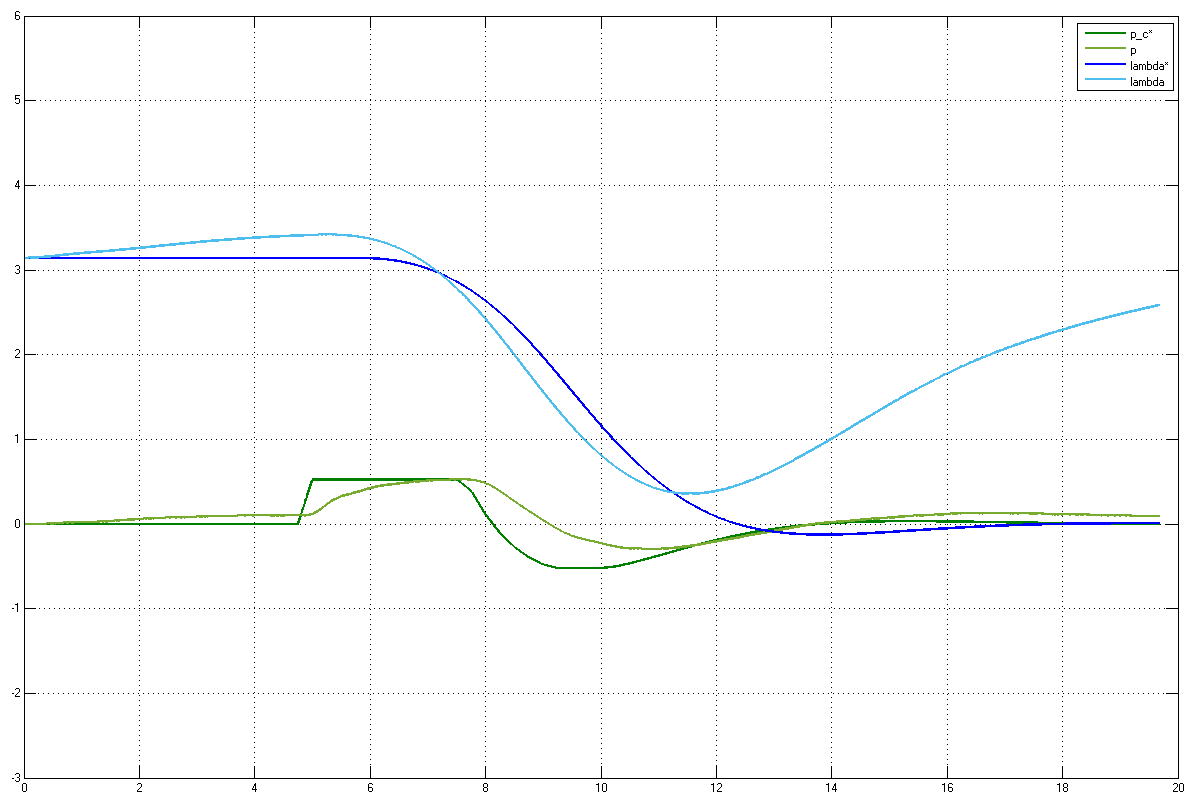
\includegraphics[width=130mm]{Part2/pitch+travel_plot_without_feedback.PNG}
    \caption{Pitch and travel response without feedback}
    \label{fig:plot_2.4}
\end{figure}

The resulting behaviour of the helicopter deviates a little from the desired trajectory. The helicopter does not end in the desired point $\boldsymbol{x_f}$ but rather a little bit earlier. The observed deviation is expected due to no feedback causing the optimization to ignore all disturbances such as friction in the hardware. Friction in the rotation may slow down the rotation compared to the estimations used in the optimization. Hence, the optimal input sequence expects the helicopter to reach the final point after a smaller amount of time than the real case. Also, our model is linearized and discretized. From experience it is known that very few systems are linear in reality. Hence a deviation necessarily occurs and increases with the distance from the linearization point. All real systems are also continuous. Hence, a deviation necessarily occurs due to the discretization in the gap between each time sample. 

Unlike pitch, the travel is not controlled with an inner controller in the basic control layer, which leads to additional deviations. Because of this, there is no control for the travel rate either. In addition, the cost function only takes into account the term $(\lambda_i - \lambda_f)$. This can result in the helicopter reaching the desired point $\lambda = \lambda_f$, but not stopping there as it should. This unwanted effect is very clear in the travel plot in figure \ref{fig:plot_2.4}.



%----------------------------------------------------------------------------------
%//////////////////////////////////////////////////////////////////////////////////
%----------------------------------------------------------------------------------


\section{Part 3: Optimal Control of Pitch/Travel with Feedback (LQ)}

\begin{figure}[H]
    \centering
    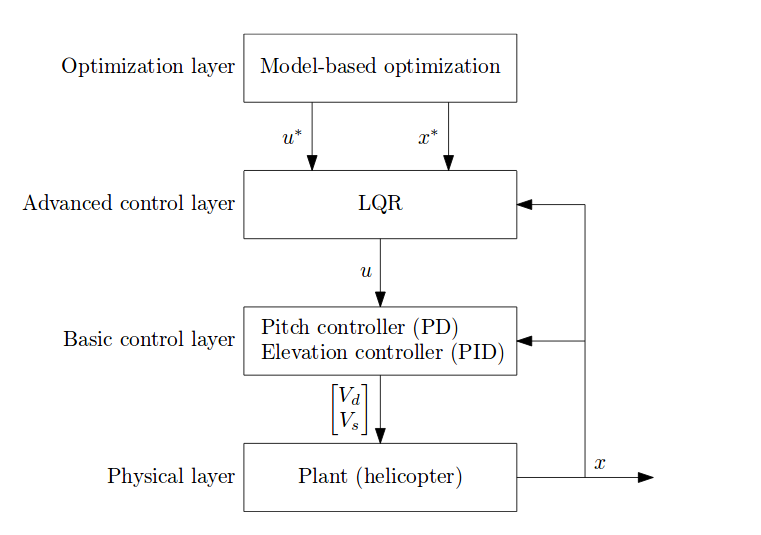
\includegraphics[width=140mm]{Part3/feedback_to_LQR.png}
    \caption{Control hierarchy }
    \label{fig:chart_3.1}
\end{figure}


\subsection{Linear Quadratic (LQ) Controller}
A new control hierarchy is shown in figure \ref{fig:chart_3.1}. In this part, an advanced control layer is added to the previous control layer. This layer uses an LQ controller to minimize a quadratic criteria for the linear model. In addition to the optimal trajectory $x_{k}^*$ and the corresponding optimal input sequence $u_{k}^*$, the manipulated variable $u_{k}$ is now adjusted due to feedback as given in equation \ref{eq:LQ_u} below.

\begin{equation}\label{eq:LQ_u}
    u_k=u_k^*-\boldsymbol{K}^T(\boldsymbol{x_k}-\boldsymbol{x_k}^*)
\end{equation}

As long as the system follows the optimal trajectory the optimal input sequence is implemented. If a deviation from $x^*$ is observed, the manipulated variable $u_k$ will be modified by the feedback term. The gain matrix K is being calculated as an LQ controller, that is minimizing the quadratic objective function

\begin{equation}\label{eq:LQ_cost}
    J=\sum_{n=1}^{\infty}\Delta\boldsymbol{{x_{i+1}}^T}\boldsymbol{Q}\Delta\boldsymbol{{x_{i+1}}} + \Delta{u_i}^TR\Delta{u_i}, \begin{tabular}{cc}
         &  \\
         & 
    \end{tabular} \boldsymbol{Q}\geq0, \quad R\geq 0
\end{equation}

for the linear model 

\begin{equation}
    \Delta\boldsymbol{{x_{i+1}}}=\boldsymbol{A}\Delta\boldsymbol{{x_i}}+\boldsymbol{B}
\end{equation}

without including inequality constraints. Here, $\Delta\boldsymbol{{x}}$ and $\Delta{u}$ are deviations from the optimal trajectory, 

\begin{equation}
    \Delta\boldsymbol{{x}}=\boldsymbol{x}-\boldsymbol{x}^* \quad \Delta{u}=u-u^*
\end{equation}

$\boldsymbol{Q}$ is chosen to be a diagonal matrix. This way each value on the diagonal could be directly related  to each state. $R$ is scalar and the last part of the cost function is therefore simple. The values in matrix $\boldsymbol{Q}$ determine how much a deviation in a particular state should be penalized and the value of $R$ determines how "expensive" the use of the manipulated variable $\boldsymbol{u_k}$ is. In practice this implies that increasing the values of $\boldsymbol{Q}$ results in increased control, while increasing $R$ limits the control. Hence increasing $\boldsymbol{Q}$ is similar to decreasing $R$. 

This is kept in mind while choosing a staring point for the values of these these parameters. The main motive of this control layer is to make the helicopter end in the desired point $\lambda_f$. Hence, deviation in travel should be penalized the most. The speed of the travel is not very important in this problem. The second value is therefore set relatively low. The travel is dependant on the pitch. Deviations in pitch is there also of certain importance, while the pitch rate has less affection.  

The feedback is implemented in Simulink as shown in figure \ref{fig:sim3_sub}. $\boldsymbol{Q}$ and $R$ is now tuned until the desired behaviour is obtained. The final $\boldsymbol{Q}$ and $R$ the the applied advanced control layer is given in \ref{eq:LQ_Q_R}.


\begin{equation} \label{eq:LQ_Q_R}
    \boldsymbol{Q}=
    \begin{bmatrix}
    50  &   0   &   0   &   0   \\
    0   &   1   &   0   &   0   \\
    0   &   0   &   10  &   0   \\
    0   &   0   &   0   &   1   \\
    \end{bmatrix}
    , \quad R=1
\end{equation}

To calculate the optimal $\boldsymbol{K}$ matrix in the controller (\ref{eq:LQ_u}) the MATLAB function dlqr is used. This function uses the chosen $\boldsymbol{Q}$ and $R$ from the cost function (\ref{eq:LQ_cost}). The resulting $\boldsymbol{K}$ is given in \ref{eq:LQ_K}.

\begin{equation} \label{eq:LQ_K}
    \boldsymbol{K}=
    \begin{bmatrix}
    -3.5745 &       0       &       0       &       0   \\
    0       &       -8.2275 &       0       &       0   \\
    0       &       0       &       3.7567  &       0   \\
    0       &       0       &       0       &       0.9578\\
    \end{bmatrix}
\end{equation}


The resulting pitch and travel response is shown in figure \ref{fig:plot_3}. Comparing this plot to the one in the last section, it is clear that the travel follows the optimal trajectory and stays in the desired point due to the feedback.

\begin{figure}[H]
    \centering
    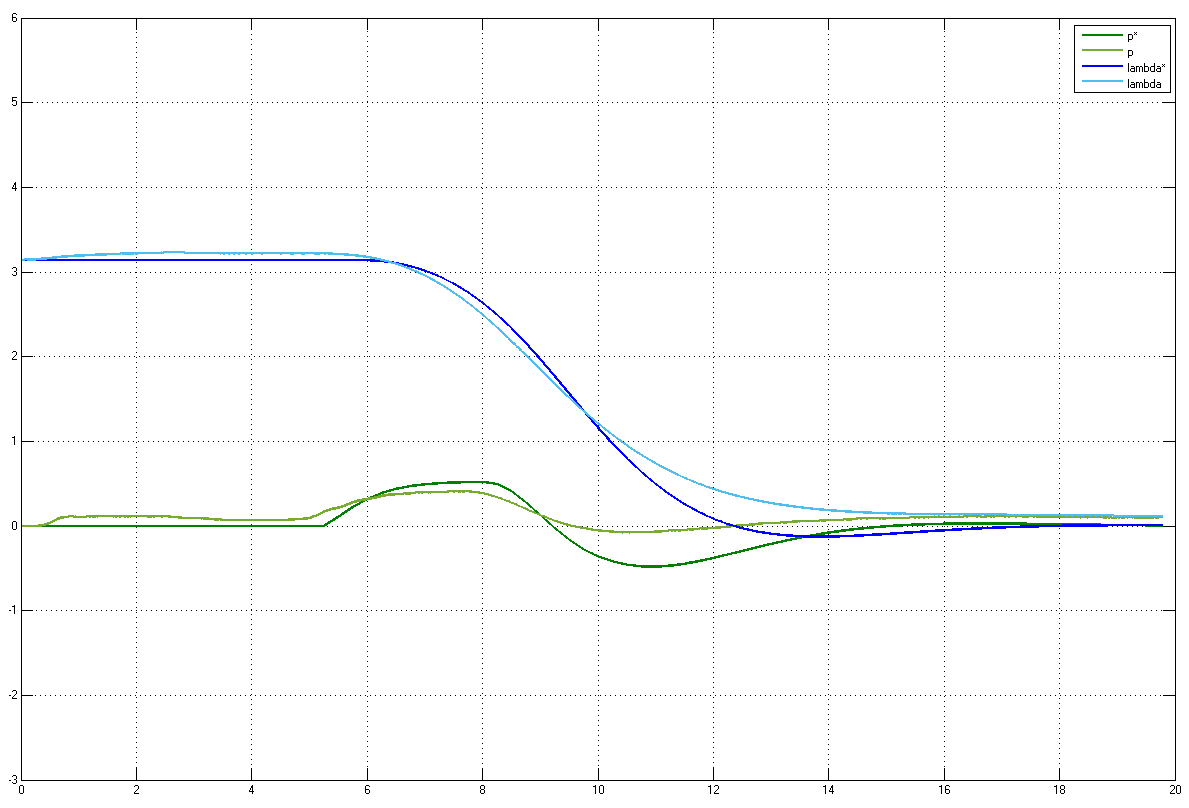
\includegraphics[width=130mm]{Part3/pitch+travel_plot_with_feedback.PNG}
    \caption{Pitch and travel response with feedback}
    \label{fig:plot_3}
\end{figure}

\subsection{Model Predictive Control(MPC)}
An alternative strategy to LQ, taking advantage of feedback, is model predictive control (MPC). MPC is repeated optimization using feedback to access the current state of the system and using this as the new initial point in every optimization.

More in depth, MPC is a form of control where the current control action is obtained by solving a finite or even infinite horizon open loop optimal control problem at every time step. The current state of the plant is as mentioned used as the initial state in every step. Each optimization outputs a new optimal input sequence $u_{k}^*$ for a finite time horizon forward in time. However, only the first of these control inputs is applied to the system before $u_{k}^*$ is recomputed and reapplied. Hence, instead of using a precalculated control gain to  adjust the control input, like the LQ controller, MPC recomputes the entire optimization, as described in the previous part, in each loop. \citep{ResearchGate}

An advantage of MPC compared to LQ is the control in a receding time window. MPC therefore allows real-time optimization against hard constraints. The main disadvantage is however the computational complexity. LQ allows a much simpler design regarding the amount and the complexity of calculations required for realization. However, the LQ controller does not handle any constraints on states and input. 


Adding MPC control to the control hierarchy in part 2 could easily be illustrated by adding an arrow from the output of the plant all the way back to the optimization layer, representing the feedback. No additional control layer is needed. Figure \ref{fig:chart_3.2} shows the control hierarchy containing MPC. \citep{Wikipedia}

\begin{figure}[H]
    \centering
    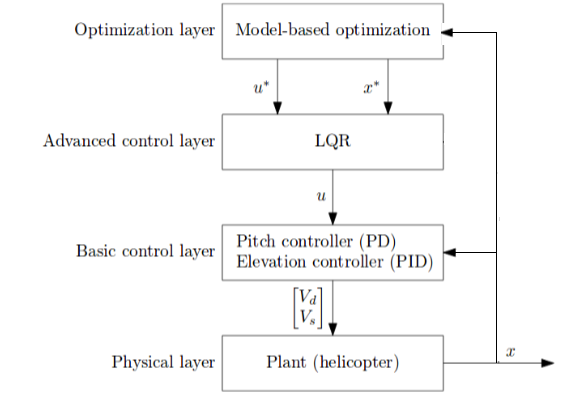
\includegraphics[width=140mm]{Part3/part32MPC.PNG}
    \caption{Control hierarchy containing MPC}
    \label{fig:chart_3.2}
\end{figure}


\section{Part 4: Optimal Control of Pitch/Travel and Elevation with
and without Feedback}


\subsection{State space model}
In this section, the desired trajectory includes two dimensions. The helicopter should now move from $x_0$ to $x_f$ past an imaginary obstacle. Hence, a change in elevation angle is necessary to avoid collision. The states $e$ and $\dot{e}$ and the input $e_c$ are therefore in this section added to the state space model. The new state- and input vector is shown in equation \ref{eq:part4_x_u}.

\begin{equation}\label{eq:part4_x_u}
    \boldsymbol{x}=\begin{bmatrix}
    \lambda\\
    r\\
    p\\
    \dot{p}\\
    e\\
    \dot{e}\\
    \end{bmatrix}, 
    \begin{tabular}{cc}
         &  \\
         & 
    \end{tabular}
    \boldsymbol{u}\begin{bmatrix}
    p_c\\
    e_c\\
    \end{bmatrix}
\end{equation}
Figure \ref{eq:state_space_extended} and shows the system written on continuous state space form having the elevation dimension included. The model matrices are determined using the model equations in equation set \ref{model_eq}

\begin{equation}\label{eq:state_space_extended}
     \begin{bmatrix}
    \dot{\lambda}\\
    \dot{r}\\
    \dot{p}\\
    \ddot{p}\\
    \dot{e}\\
    \ddot{e}\\
    \end{bmatrix} = 
    \begin{bmatrix}
    0 & 1 & 0 & 0 & 0 & 0\\
    0 & 0 & -K_2 & 0 & 0 & 0\\
    0 & 0 & 0 & 1 & 0 & 0\\
    0 & 0 & -K_1K_{pp} & -K_{1}K_{pd} & 0 & 0\\
    0 & 0 & 0 & 0 & 0 & 1\\
    0 & 0 & 0 & 0 & -K_3K_{ep} & -K_3K_{ed}\\
    \end{bmatrix} 
    \begin{bmatrix}
    \lambda\\
    r\\
    p\\
    \dot{p}\\
    e\\
    \dot{e}\\
    \end{bmatrix} + 
    \begin{bmatrix}
    0 & 0\\
    0 & 0\\
    0 & 0\\
    K_1K_{pp} & 0\\
    0 & 0\\
    0 & K_3K_{ep}\\
    \end{bmatrix} 
    \begin{bmatrix}
    p_c\\
    e_c\\
    \end{bmatrix}
 \end{equation}  


\subsection{Discretization}
The new continuous model is once again discretized using the forward Euler method similar to section 3.2. The new extended discret state space model is given in  in the matrices in equation \ref{eq:discA}.

\begin{equation}\label{eq:discA}
    \begin{aligned}
        \begin{bmatrix}
            \lambda_{k+1}\\
            r_{k+1}\\
            p_{k+1}\\
            \dot{p}_{k+1}\\
            e_{k+1}\\
            \dot{e}_{k+1}\\
        \end{bmatrix} &= 
        \begin{bmatrix}
            1 & \Delta{t} & 0 & 0 & 0 & 0\\
            0 & 1 & -\Delta{t}K_2 & 0 & 0 & 0\\
            0 & 0 & 1 & \Delta{t} & 0 & 0\\
            0 & 0 & -\Delta{t}K_1K_{pp} & 1-\Delta{t}K_{1}K_{pd} & 0\\
            0 & 0 & 0 & 0 & 1 & \Delta{t}\\
            0 & 0 & 0 & 0 & -\Delta{t}K_3K_{ep} & -\Delta{t}K_3K_{ed}+1\\
        \end{bmatrix} 
        \begin{bmatrix}
            \lambda\\
            r\\
            p\\
            \dot{p}\\
            e\\
            \dot{e}\\
        \end{bmatrix} \\
        &+ \begin{bmatrix}
            0 & 0\\
            0 & 0\\
            0 & 0\\
            \Delta{t} K_1K_{pp} & 0\\
            0 & 0 \\
            0 & \Delta{t}K_3K_{ep}
        \end{bmatrix} 
        \begin{bmatrix}
            p_c\\
            e_c\\
        \end{bmatrix}
    \end{aligned}
\end{equation}


\subsection{Optimization problem with nonlinear constraints}
An inequality constraint is now implemented on the elevation. This constraint represents the imaginary obstacle that the helicopter should pass. The nonlinear constraint is given in equation \ref{obst_con} below. 

\begin{equation}\label{obst_con}
    e_k \geq \alpha \exp(-\beta (\lambda_k - \lambda_t) ), \quad \forall k\in [1,....,N]
\end{equation}
 
The QP solver used in \texttt{quadprog} only solves problem with linear constraints. Since the new problem contains an additional nonlinear constraint, the MATLAB function \texttt{fmincon} is used instead. The criteria to be minimized is now, 
 
\begin{equation}
    \Phi=\sum_{i=1}^{N}(\lambda_i-\lambda_f)^2+q_1p_{ci}^2+q_2e_{ci}^2, \quad q\geq 0
\end{equation}
 
The following values are used: $q_1=q_2=1$, $\alpha=0.2$, $\beta=20$, $\lambda_t=\frac{2\pi}{3}$, $\Delta{t}=0.25 s$.
For every point in time a constraint on the form 

\begin{equation}
    c(x_k)=\alpha exp(-\beta(\lambda_k - \lambda_t)^2)-e_k\geq0
\end{equation}

is implemented as a function named "nonlcon" and passed to the \texttt{fmincon}.This is seen in \ref{script:4}. The first attempt of using \texttt{fmincon} function was with the active set method. However, this method could get stuck in a local minimum. The method is therefore changed to SQP, which stands for Sequential Quadratic Programming. Since this is a quadratic problem the SQP is a more suitable solver. 
 
\subsection{Applying LQ control using feedback}\label{5.4}

The LQ controller is once again used to adjust the input setpoints originally calculated in the optimization layer, using feedback control. The responses of the system without feedback is given in figure \ref{fig:plot_4.1}. As the plot illustrates, the optimization layer alone does not propose the desired behaviour. The most significant misbehaviour is the deviation of the travel angle from its reference. The elevation angle also stays close to zero during the entire sequence and even below zero for a period of time. Considering the imaginary obstacle, the elevation angle should increase significantly more in order to pass without collision.

 The purpose of applying LQ using feedback control is hence to improve the behaviour and make it as close as possible to the optimal trajectory. Applying feedback leads to a quick recognization of the tendency of "moving off track". This is furthermore effectively handled before the deviations becomes significant. 



\begin{figure}[H]
    \centering
    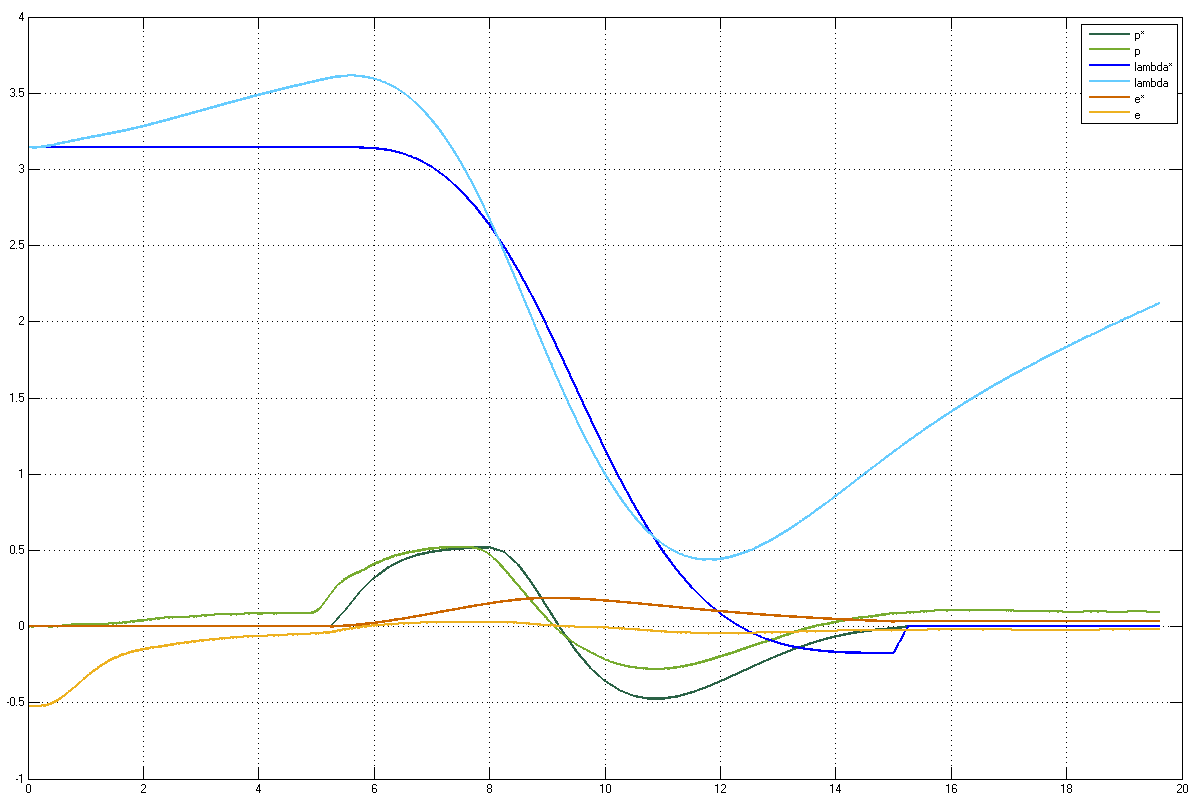
\includegraphics[width=150mm]{Part4/without_feedback_bad_tuning.PNG}
    \caption{Pitch, travel and elevation response without feedback}
    \label{fig:plot_4.1}
\end{figure}

 The effect of the feedback depends on the tuning of the LQ-controller. In practice, this implies tuning of the weights in the \boldsymbol{Q} matrix. To achieve an improved behaviour as close as possible to the desired trajectory, the first attempt of tuning the \boldsymbol{Q} matrix of the applied controller is given in \ref{eq:Q_bad}. This matrix is used as input in the MATLAB function \texttt{dlqr} to determine the corresponding gain matrix \boldsymbol{K} which is directly taken into use in the feedback controller. The resulting behaviour is shown in figure \ref{fig:plot_4.2} below. 

\begin{equation}
    \label{eq:Q_bad}
    \boldsymbol{Q} = 
    \begin{bmatrix}
        10 & 0 & 0 & 0 & 0 & 0 \\
        0 & 1 & 0 & 0 & 0 & 0 \\
        0 & 0 & 0 & 0 & 0 & 0 \\
        0 & 0 & 0 & 0 & 5 & 0 \\
        0 & 0 & 0 & 0 & 0 & 0 \\
    \end{bmatrix}
\end{equation}

\begin{figure}[h!]
    \centering
    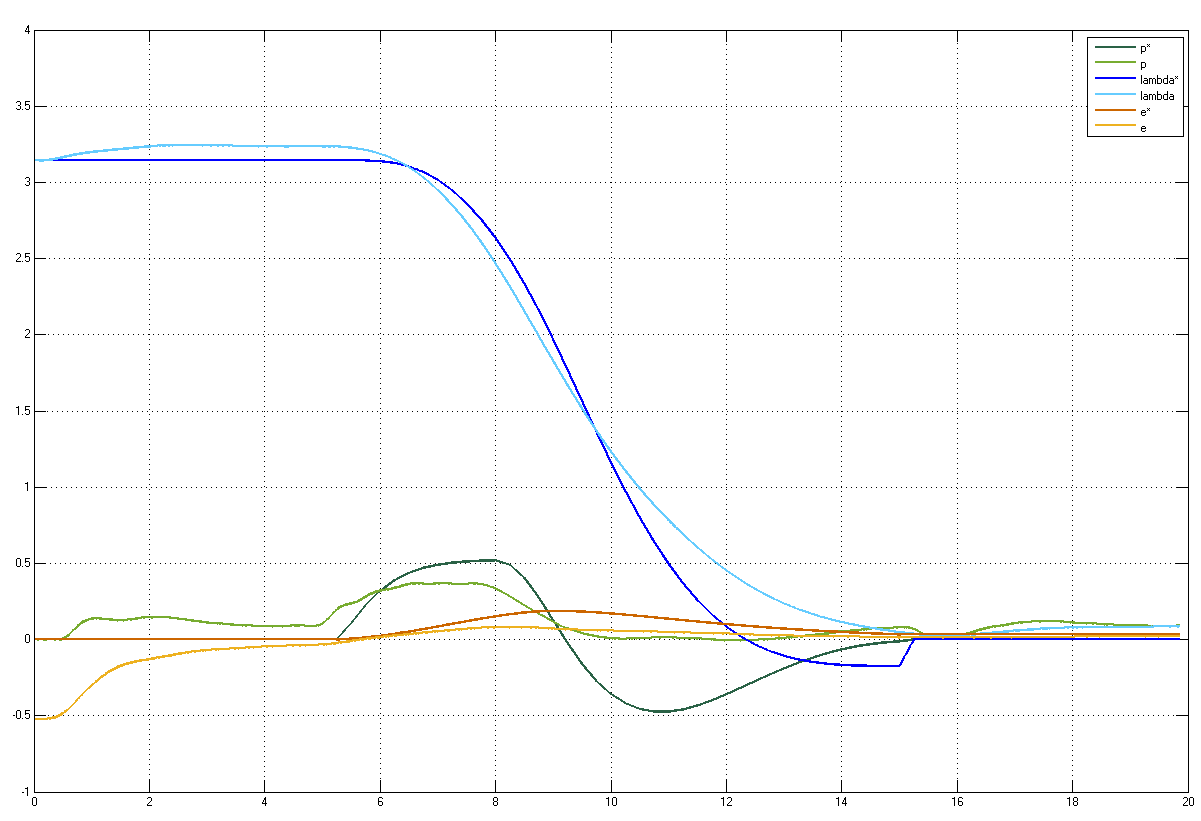
\includegraphics[width=150mm]{Part4/with_feedback_bad_tuning.PNG}
    \caption{Pitch, travel and elevation response with feedback}
    \label{fig:plot_4.2}
\end{figure}

As mentioned, the different weights in the $\boldsymbol{Q}$ of an LQ-controller represent how much a deviation between measured and estimated state should be punished, relative to the other states. The chosen values in \ref{eq:Q_bad} implies that an error in the travel state should be punished the most. This is connected to the great deviations in travel observed in the previous plot (\ref{fig:plot_4.1}) without feedback. The travel is consequently considerably better with the feedback control, and is no longer steering away from the optimal travel in the end of the sequence. Furthermore, error in the elevation is also punished a certain amount. This is however only weighted half the amount of the travel state weight. The result is a relatively small improvement compared to not having feedback control, and it is still expected that the helicopter would collide with the obstacle.

To pass the obstacle, it is necessary to increase the weighting of deviation in  the elevation state. The helicopter is therefore further tuned keeping this in mind. The resulting final \boldsymbol{Q} matrix is given in \ref{eq:Q_good}. As shown, the weight connected to the elevation state is increased to 30, which is significantly higher than the other weights. 

\begin{equation}
    \label{eq:Q_good}
    \boldsymbol{Q} = 
    \begin{bmatrix}
        10 & 0 & 0 & 0 & 0 & 0 \\
        0 & 1 & 0 & 0 & 0 & 0 \\
        0 & 0 & 0 & 0 & 0 & 0 \\
        0 & 0 & 0 & 0 & 30 & 0 \\
        0 & 0 & 0 & 0 & 0 & 0 \\
    \end{bmatrix}
\end{equation}

The resulting behaviour of the helicopter is shown in figure \ref{fig:plot_4.3}.  The elevation is now following the reference better than in the previous plots. However, the optimal trajectory is determined by solving an optimization problem. It therefore represents the shortest path passing the nonlinear constraint. This means that the helicopter has to have an elevation greater than or equal to the optimal elevation in order to avoid the obstacle. The behaviour shown in \ref{fig:plot_4.3} would therefore probably still lead to collision with the obstacle. However, increasing the weight of the elevation furthermore quickly lead to the controller caring too little about the other states as these weight became very low in relation. These challenges should be possible to solve by simply spend some time tuning all the weights on a finer level.

\begin{figure}[h!]
    \centering
    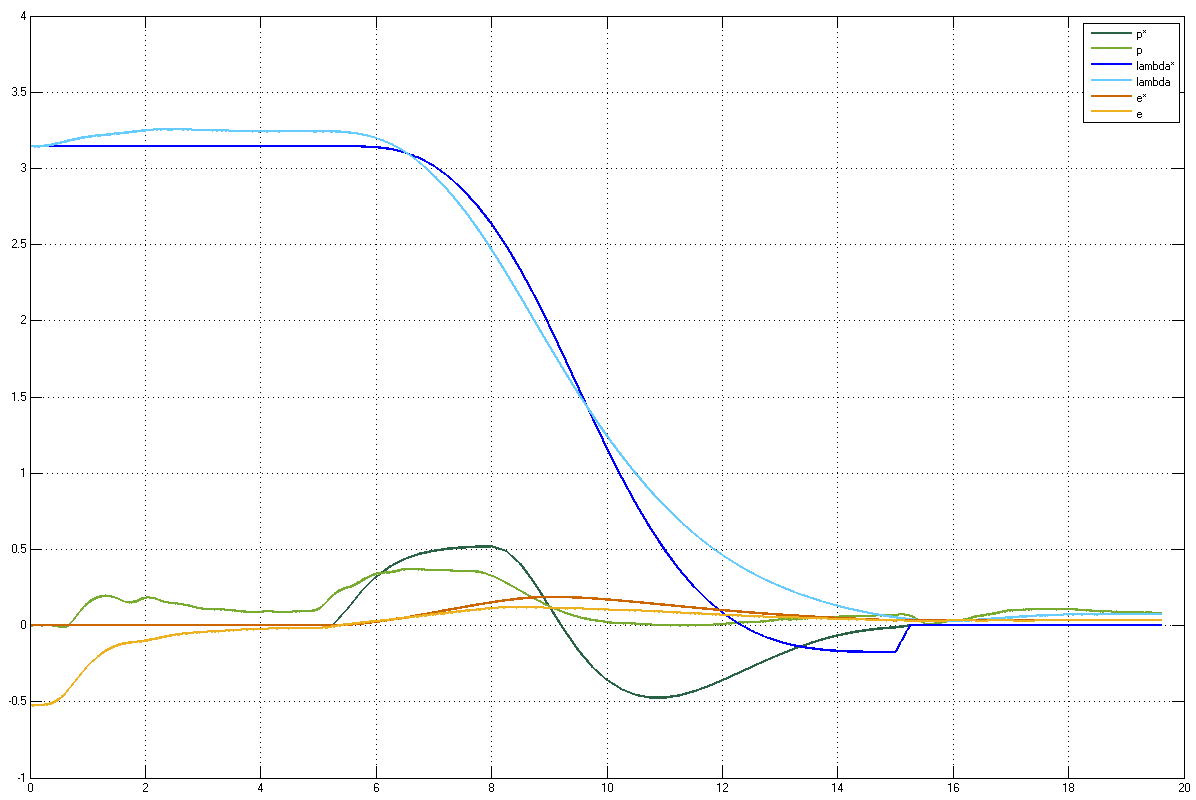
\includegraphics[width=150mm]{Part4/with_feedback_better_tuning.PNG}
    \caption{Pitch, travel and elevation response with feedback}
    \label{fig:plot_4.3}
\end{figure}

It can be noticed that the pitch is actually worse in the cases with feedback than in the case without feedback. Nor is any weight added to the LQ to try and compensate for this. This is because there is no constraint on the pitch angle. The pitch is only used to steer the elevation and travel to the right values. The fact that the pitch differs more from the optimal pitch when the other states are more accurate, indicates that the input sequence for the pitch is not really optimal.


\subsection{Decoupled states}
The first four states in the model are completely decoupled from the last two. This means that changing the pitch would not affect the elevation of the helicopter, which is not the case in reality.

The observed behaviour of the elevation in the previous section could be explained by the simplifications used in the model. The model equation describing the dynamics of the elevation is derived assuming zero pitch angle. However, in this case, the elevation has to change simultaneously with the changing travel. The travel requires a pitch angle, resulting in the force from the helicopter motors no longer pointing all upwards, but rather having a force component in the horizontal plane as well.\\
A solution to this problem would be to improve the model, ensuring coupling between all states. This could be achieved by making less simplifications in the mathematical model, which could result in an non-linear model. 

\section{Discussion}

This laboratory exercise is useful for distinguishing the different control methods and understanding the application, advantages and disadvantages of each method. Optimization is necessary when the desired behaviour of a system is defined by certain constraints. This is because optimization allows inclusion of constraints in its calculations and outputs an optimal trajectory defining the concrete desired behaviour that is indirectly given by the constraints together with the objective function to be minimized. Hereafter, it also calculates a sequence of input setpoints that should propose the system to develop in order to the optimal trajectory. 

However, as seen there are some weaknesses to this method. The model based optimization is based only on the given model. As several assumptions are made when making this model, it does not represent the physical behaviour of the system accurately. This means that the optimal input sequence will be optimal in theory, but not necessarily in practice. The solution is to introduce a new control layer to the hierarchy - LQ control. This controller takes advantage of feedback to compare the optimal and actual states, and uses the result to modify the input so that it compensates for the errors from the model-based optimization. The LQ controller is especially useful when the desired behaviour poses stronger requirements for some states rather than others. This is very often the case. The LQ allows weighting of the different states, so that punishment of detected errors in each state becomes prioritized. However, the error was not cancelled out completely in this exercise. Better tuning of the LQ controller and a better model for the physical system that takes into account the relation between elevation and pitch would most probably be the solution to these challenges.



\newpage

\section{Appendix A: Plots}
\subsection{Part 2}

\begin{figure}[H]
    \centering
    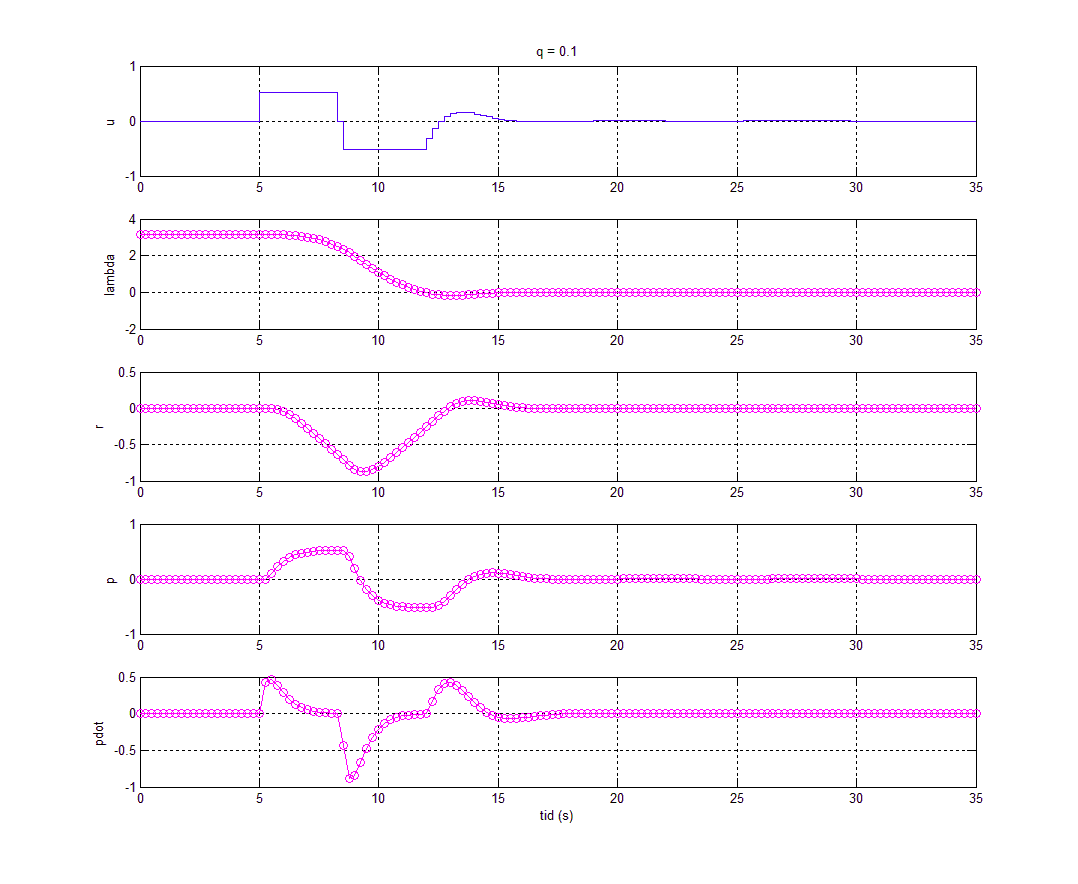
\includegraphics[width=150mm]{Part2/q_lik_0_komma_1.png}
    \caption{Weight $q$ = 0.1}
    \label{fig:plot_2.3_1}
\end{figure}

\begin{figure}[H]
    \centering
    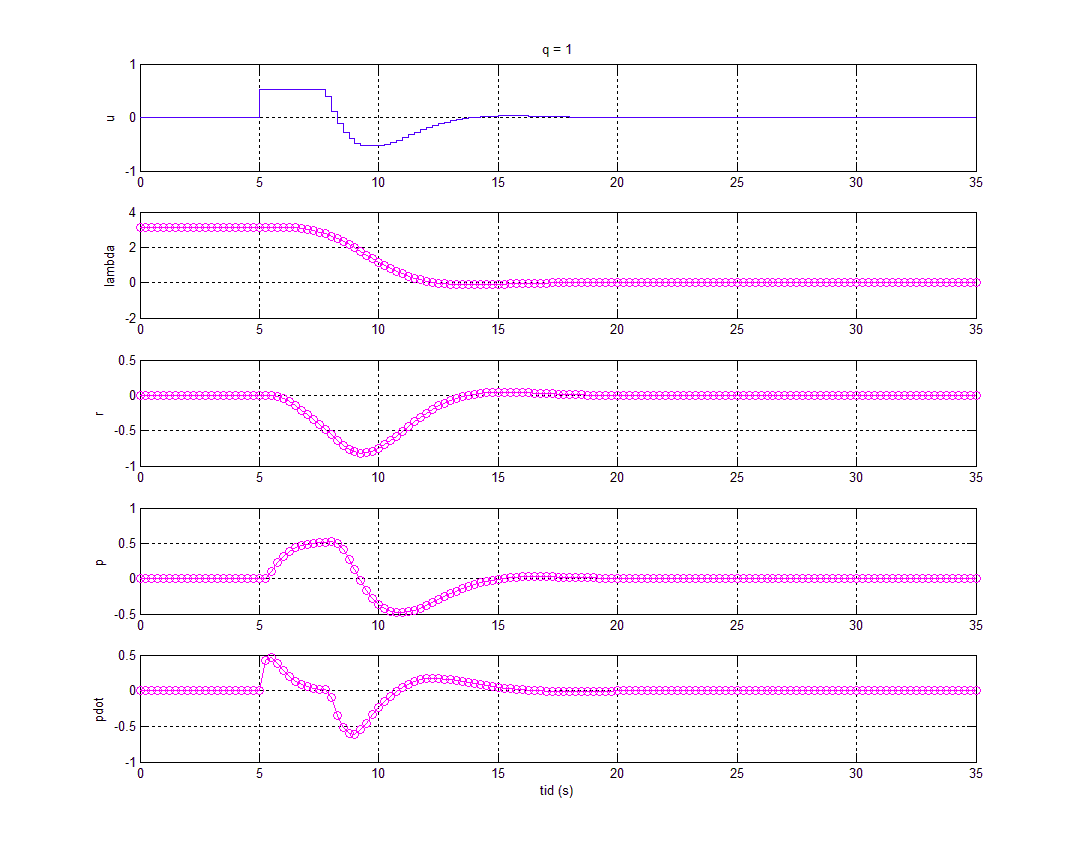
\includegraphics[width=150mm]{Part2/q_lik_1.png}
    \caption{Weight $q$ = 1}
    \label{fig:plot_2.3_2}
\end{figure}

\begin{figure}[H]
    \centering
    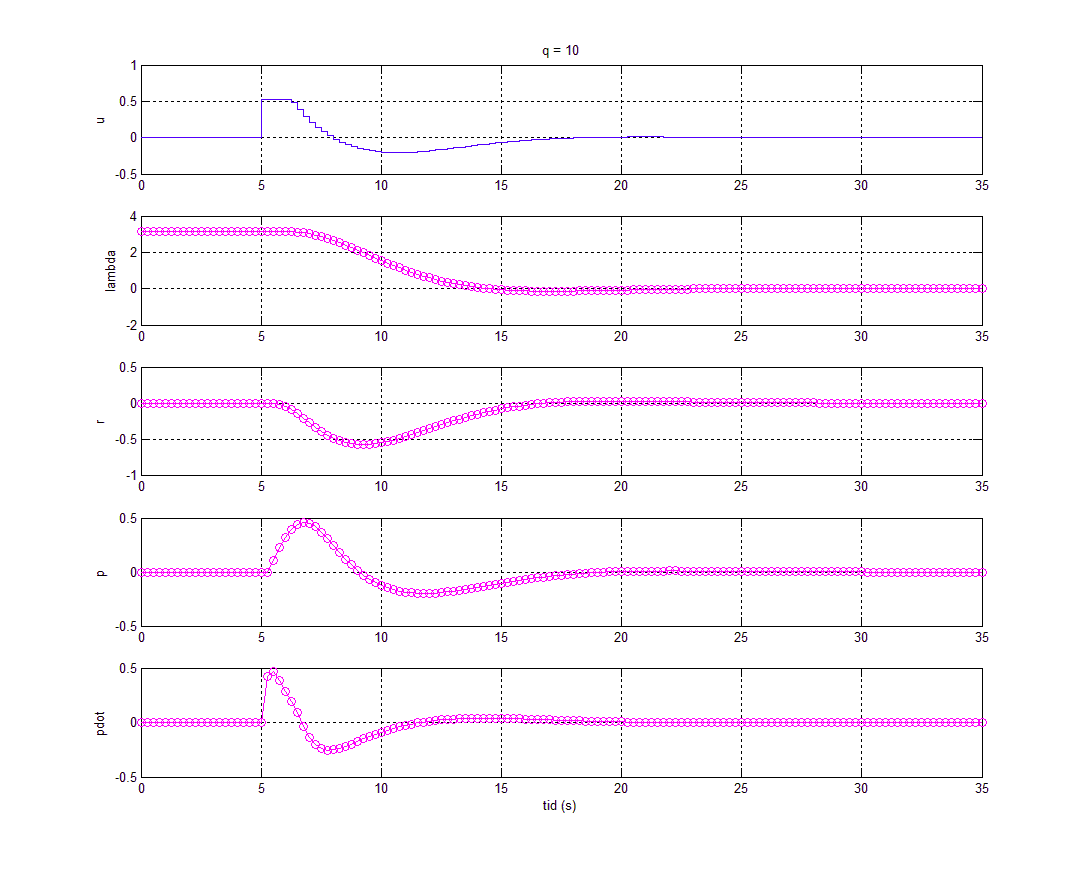
\includegraphics[width=150mm]{Part2/q_lik_10.png}
    \caption{Weight $q$ = 10}
    \label{fig:plot_2.3_3}
\end{figure}



\section{Appendix B: MATLAB scripts}

\subsection{Script part 2}
\lstinputlisting[language=Octave]{Scripts/Part2.m}

\subsection{Script part 3}
\lstinputlisting[language=Octave]{Scripts/part3.m}

\subsection{Script part 4} \label{script:4}
\lstinputlisting[language=Octave]{Scripts/part4.m}

\section{Simulink Diagrams}

\begin{figure}[H]
    \centering
    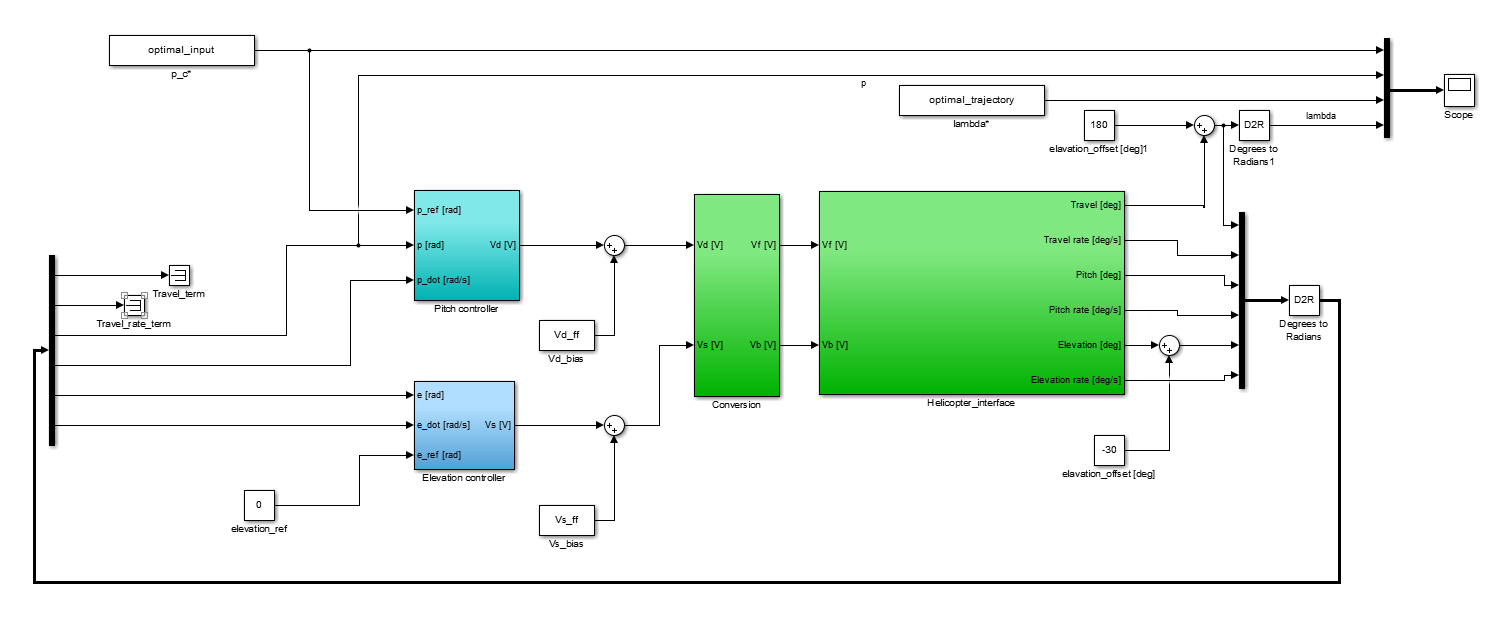
\includegraphics[width=150mm]{Part2/simulink_part2.PNG}
    \caption{Simulink part 2}
    \label{fig:sim2}
\end{figure}

\begin{figure}[H]
    \centering
    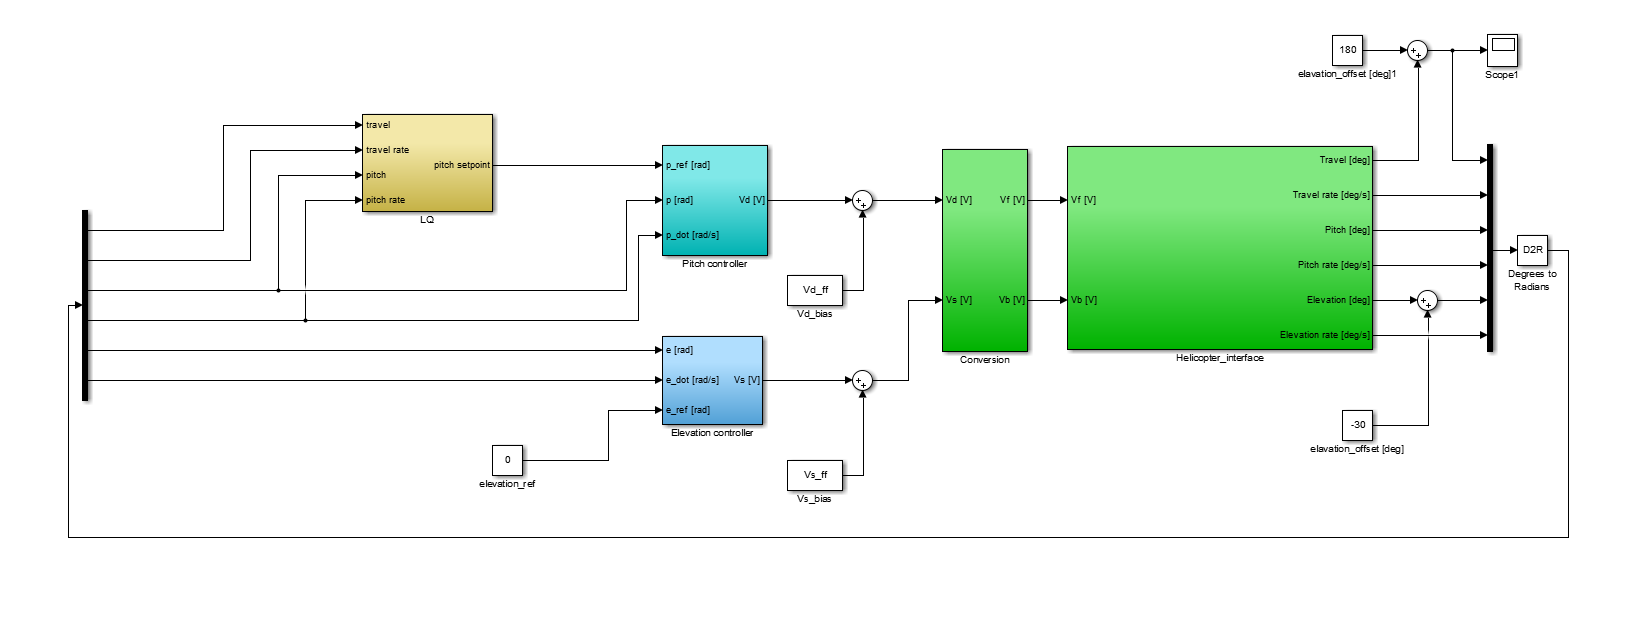
\includegraphics[width=150mm]{Part3/simulink_part3.PNG}
    \caption{Simulink part 3}
    \label{fig:sim3}
\end{figure}

\begin{figure}[H]
    \centering
    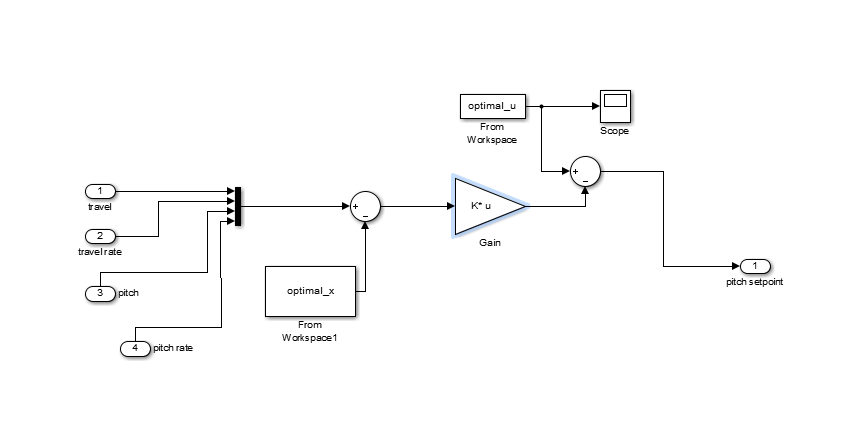
\includegraphics[width=150mm]{Part3/simulink_LQsubsystem_part3.PNG}
    \caption{Simulink part 3, LQ subsystem}
    \label{fig:sim3_sub}
\end{figure}

\begin{figure}[H]
    \centering
    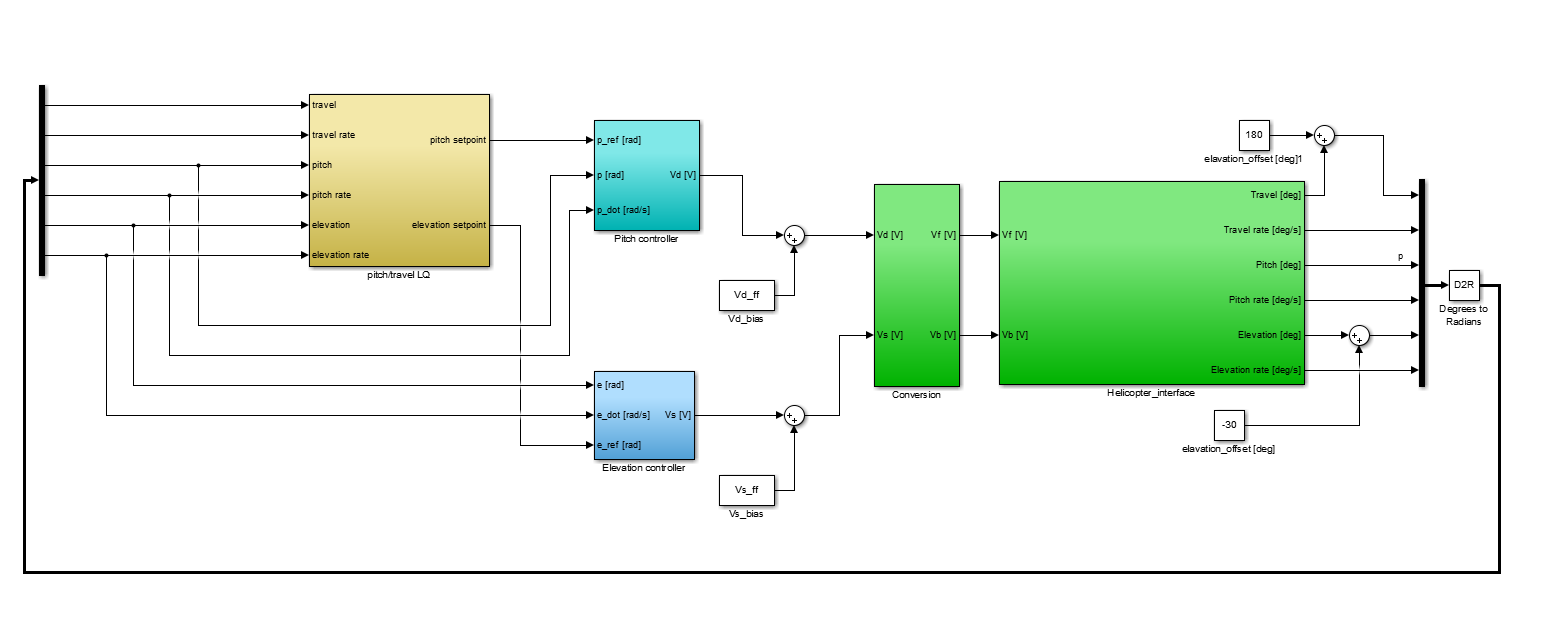
\includegraphics[width=150mm]{Part4/simulink_part4.PNG}
    \caption{Simulink part 4}
    \label{fig:sim4}
\end{figure}

\begin{figure}[H]
    \centering
    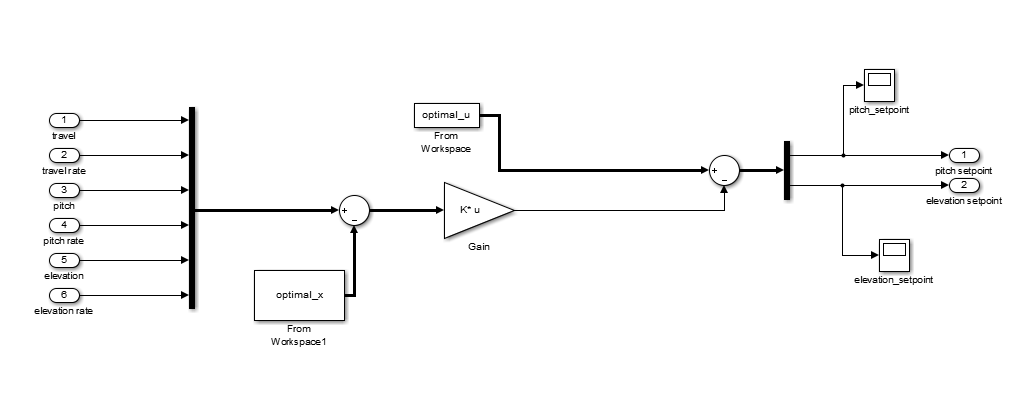
\includegraphics[width=150mm]{Part4/LQ_with_feedback_part4.PNG}
    \caption{Simulink part 4, LQ subsystem with feedback}
    \label{fig:sim4_sub1}
\end{figure}

\begin{figure}[H]
    \centering
    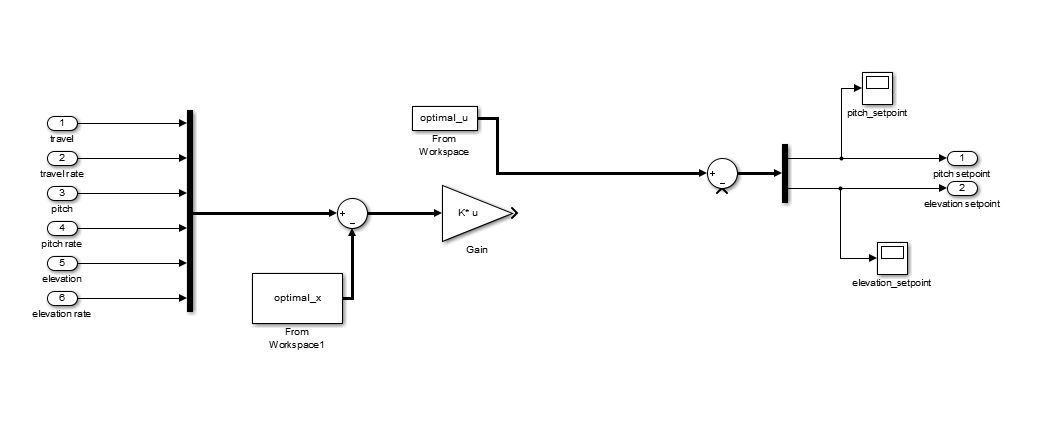
\includegraphics[width=150mm]{Part4/LQ_without_feedback_part4.PNG}
    \caption{Simulink part 4, LQ subsystem without feedback}
    \label{fig:sim4_sub2}
\end{figure}

\addcontentsline{toc}{section}{References}
\bibliographystyle{plain}
\bibliography{references}


\end{document}
